\section{Quy trình tổng quan}

Mục tiêu của công cụ là phân tích mã nguồn Rust và xây dựng đồ thị thuộc tính mã
nguồn (CPG) biểu diễn mã nguồn đó. Hình 3.1 thể hiện các bước xây dựng cây CPG từ
các tệp mã nguồn Rust.

\begin{figure}[H]
	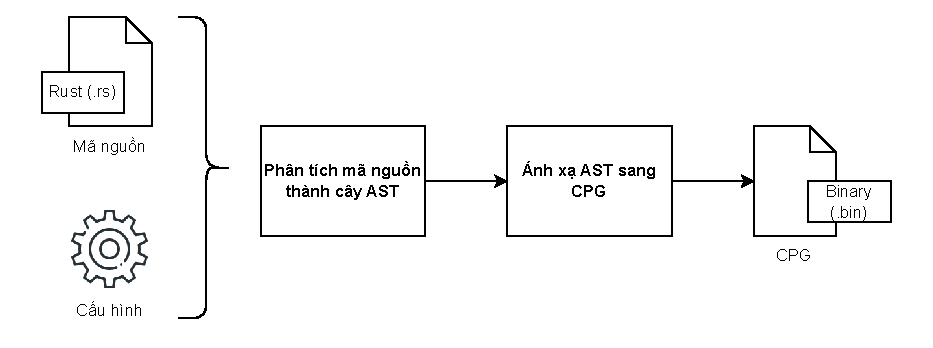
\includegraphics[width=1\columnwidth]{figures/c3/c3_flow.drawio.pdf}
	\centering
	\caption{Quy trình phân tích mã nguồn Rust}
	\label{img:method_flow}
\end{figure}

Mã nguồn Rust sẽ được trình phân tích go/parser phân tích và sinh ra cây AST tương
ứng với từng tệp mã nguồn. Sau đó, công cụ go/package sẽ phân tích các tệp mã nguồn
và sinh ra các thông tin về kiểu dữ liệu và ta sẽ thực hiện bổ sung các thông tin về kiểu dữ
liệu và một số thông tin khác như chữ ký (signature), tên đầy đủ (fullyQualifiedName) và kiểu dữ liệu vào các nút tương ứng trong cây cú pháp trừu tượng. Ở bước thứ ba, cây
cú pháp trừu tượng sẽ được ánh xạ sang đồ thị thuộc tính mã nguồn. Cuối dùng, đồ thị
CPG sẽ được lưu dưới dạng cơ sở dữ liệu đồ thị phục vụ mục đích của người dùng.